%==============================================================================
%  CISC-727 — A05: Related Work Package (standalone)
%  Author: Kenneth Peter Fernandes
%  Companion to AREII_Ready_Package.tex (Part II is reproduced here as
%  a standalone artifact for the related-work deliverable.)
%==============================================================================
\documentclass[11pt]{article}

\usepackage[margin=1in]{geometry}
\usepackage[T1]{fontenc}
\usepackage[utf8]{inputenc}
\usepackage{mathptmx}
\usepackage{setspace}
\usepackage{parskip}
\usepackage{titlesec}
\usepackage{enumitem}
\usepackage{hyperref}
\usepackage{graphicx}
\usepackage{booktabs}
\usepackage{xcolor}
\usepackage{csquotes}
\usepackage{tabularx}
\usepackage{longtable}
\usepackage{array}
\usepackage{tikz}
\usetikzlibrary{trees, positioning, shapes.geometric, arrows.meta}

\usepackage[style=apa,backend=biber,sortcites=true]{biblatex}
\DeclareLanguageMapping{american}{american-apa}
\addbibresource{../proposal/references.bib}

\hypersetup{colorlinks=true, linkcolor=blue, citecolor=blue, urlcolor=blue}
\onehalfspacing

\title{%
    \textbf{Related Work Package}\\[0.3em]
    \large Literature Map, Gap Matrix, and Annotated Bibliography\\[0.5em]
    \large CISC-727 --- Advanced Research Explorations (ARE) - I\\[0.2em]
    \large Assignment A05 (Companion Artifact)
}
\author{%
    Kenneth Peter Fernandes\\
    Harrisburg University of Science and Technology
}
\date{April 25, 2026}

\begin{document}
\maketitle

\noindent\textit{This document is the standalone related-work package for Assignment A05. It reproduces the literature map, the gap matrix, and the annotated bibliography from Part~II of \texttt{AREII\_Ready\_Package.tex}. Its purpose is to allow an advisor to inspect the related-work deliverable independently of the integrated bundle.}

\section{Literature Map}

The literature relevant to this work falls into six clusters: (1) the foundational Transformer baseline; (2) survey and taxonomy literature; (3) IO-aware exact attention (FlashAttention family); (4) Key-Value cache management and head-sharing for inference; (5) sparse and linear/low-rank approximate attention; and (6) benchmark and evaluation frameworks. Figure~\ref{fig:lit-map} shows the visual taxonomy in tree form.

\begin{figure}[h!]
\centering
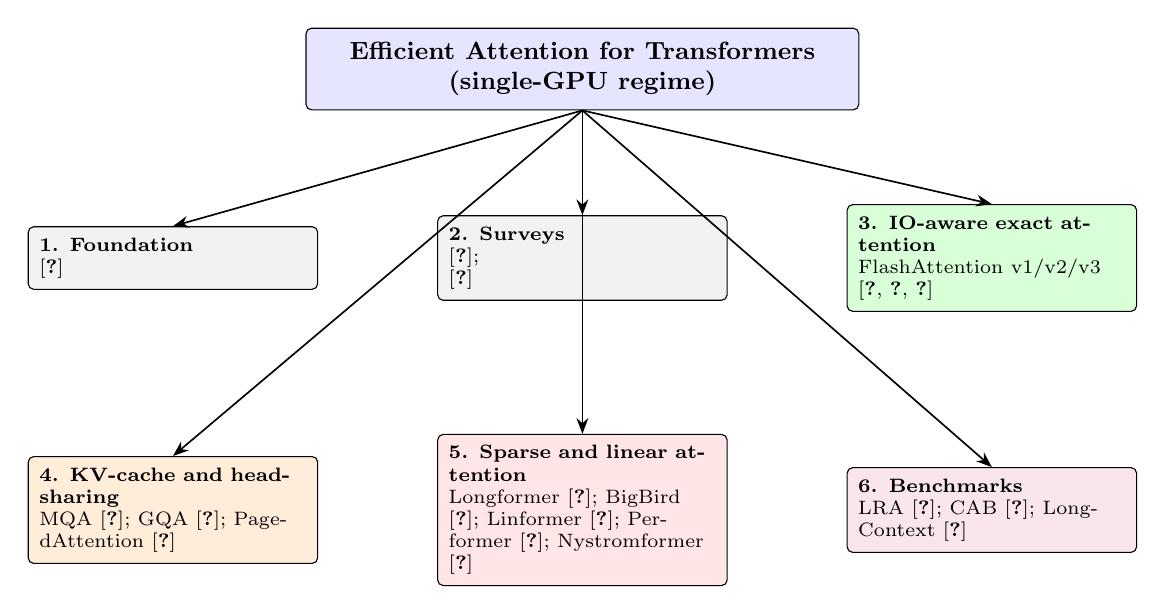
\begin{tikzpicture}[
    every node/.style={font=\scriptsize, align=left},
    box/.style={rectangle, draw, rounded corners=2pt, text width=0.28\textwidth, inner sep=4pt},
    rootbox/.style={rectangle, draw, rounded corners=2pt, fill=blue!10, text width=0.55\textwidth, align=center, inner sep=5pt, font=\small\bfseries},
]
\node[rootbox] (root) at (0,0) {Efficient Attention for Transformers\\(single-GPU regime)};

\node[box, fill=gray!10] (foundation) at (-5.2, -2.4)
  {\textbf{1. Foundation}\\
   \cite{vaswani2023attentionneed}};
\node[box, fill=gray!10] (survey) at (0, -2.4)
  {\textbf{2. Surveys}\\
   \cite{10.1145/3530811};\\
   \cite{sun2026efficientattentionmechanismslarge}};
\node[box, fill=green!15] (ioaware) at (5.2, -2.4)
  {\textbf{3. IO-aware exact attention}\\
   FlashAttention v1/v2/v3
   \cite{dao2022flashattentionfastmemoryefficientexact, dao2023flashattention2fasterattentionbetter, shah2024flashattention3fastaccurateattention}};

\node[box, fill=orange!15] (kv) at (-5.2, -5.6)
  {\textbf{4. KV-cache and head-sharing}\\
   MQA \cite{shazeer2019fasttransformerdecodingwritehead};
   GQA \cite{ainslie2023gqatraininggeneralizedmultiquery};
   PagedAttention \cite{kwon2023efficientmemorymanagementlarge}};
\node[box, fill=red!10] (sparse) at (0, -5.6)
  {\textbf{5. Sparse and linear attention}\\
   Longformer \cite{beltagy2020longformerlongdocumenttransformer};
   BigBird \cite{zaheer2021bigbirdtransformerslonger};
   Linformer \cite{wang2020linformerselfattentionlinearcomplexity};
   Performer \cite{choromanski2022rethinkingattentionperformers};
   Nystromformer \cite{xiong2021nystromformernystrombasedalgorithmapproximating}};
\node[box, fill=purple!10] (bench) at (5.2, -5.6)
  {\textbf{6. Benchmarks}\\
   LRA \cite{tay2020longrangearenabenchmark};
   CAB \cite{zhang2025cabcomprehensiveattentionbenchmarking};
   Long-Context \cite{bu2025longcontextattentionbenchmark}};

\draw[->, >=Stealth, semithick] (root.south) -- (foundation.north);
\draw[->, >=Stealth, semithick] (root.south) -- (survey.north);
\draw[->, >=Stealth, semithick] (root.south) -- (ioaware.north);
\draw[->, >=Stealth, semithick] (root.south) -- (kv.north);
\draw[->, >=Stealth, semithick] (root.south) -- (sparse.north);
\draw[->, >=Stealth, semithick] (root.south) -- (bench.north);
\end{tikzpicture}
\caption{Literature taxonomy. The proposed contribution sits at the single-GPU intersection of Cluster~3 (IO-aware exact attention) and Cluster~6 (benchmarks), specifically on Turing-class hardware that the cited literature does not cover.}
\label{fig:lit-map}
\end{figure}

\section{Gap Matrix}

Table~\ref{tab:gap-matrix} compares the closest competitors on the dimensions that matter for the proposed contribution: hardware regime evaluated, kernel actually exercised, sequence-length range, whether kernel attribution is performed, whether the Tesla T4 is covered, and the distance from the present work.

\begin{table}[h!]
\centering
\caption{Gap matrix: closest-competitor comparison on six dimensions}
\label{tab:gap-matrix}
\footnotesize
\begin{tabularx}{\textwidth}{p{2.4cm} p{1.7cm} p{2.0cm} p{1.6cm} p{1.4cm} p{1.4cm} X}
\toprule
\textbf{Work} & \textbf{Hardware regime} & \textbf{Kernel exercised} & \textbf{Seq.\ length range} & \textbf{Kernel attribution?} & \textbf{Tesla T4 covered?} & \textbf{Distance from this work} \\
\midrule
FlashAttention v1 \cite{dao2022flashattentionfastmemoryefficientexact} & A100 & FlashAttention v1 & 128--64K & Implicit & No & Reports A100 only; no T4. \\
FlashAttention v2 \cite{dao2023flashattention2fasterattentionbetter} & A100 & FlashAttention v2 & 128--16K & Implicit & No & Requires sm\_80; not runnable on T4. \\
FlashAttention v3 \cite{shah2024flashattention3fastaccurateattention} & H100 & FlashAttention v3 & 1K--16K & Implicit & No & Hopper-specific; T4 not addressed. \\
PagedAttention/vLLM \cite{kwon2023efficientmemorymanagementlarge} & Multi-GPU server & Standard attention with paged KV & 1K--32K & No & No & Targets KV memory, not kernel choice. \\
Long Range Arena \cite{tay2020longrangearenabenchmark} & TPU/GPU (varied) & Multiple & 1K--16K & No & No & Quality benchmark; not kernel-level. \\
Comprehensive Attention Benchmark \cite{zhang2025cabcomprehensiveattentionbenchmarking} & GPU (varied) & Multiple & 1K--16K & No & Implicit only & Cross-pattern quality benchmark; no T4 kernel attribution. \\
Long-Context Attention Benchmark \cite{bu2025longcontextattentionbenchmark} & Cluster up to 96 GPUs & FlashAttention v2/v3 & 4K--256K & Yes & No & Multi-GPU; data-center class only. \\
\midrule
\textbf{This work} & \textbf{Tesla T4 (Turing, sm\_75)} & \textbf{Math, memory-efficient SDPA, xFormers; FlashAttention attempted} & \textbf{64--4{,}096} & \textbf{Yes (profiler-traced)} & \textbf{Yes} & --- \\
\bottomrule
\end{tabularx}
\end{table}

\section{Top Three Identified Gaps}

\begin{enumerate}[leftmargin=2em]
    \item \textbf{No kernel-attribution evidence on the Tesla T4.} The Tesla T4 is the most widely available free-tier accelerator for graduate research, but no published study reports which CUDA kernel is actually launched when an SDPA backend is requested on it. The pilot evidence from A03 and A04 motivates the concern: results labelled \enquote{flash} may have measured a fallback kernel.
    \item \textbf{No single-GPU, Turing-class crossover map.} The published FlashAttention crossover analyses target Ampere (A100) or Hopper (H100). The Comprehensive Attention Benchmark reports \emph{efficiency length} but on cross-pattern quality rather than on T4 kernel times. The 2025 Long-Context Attention Benchmark addresses kernel time but on multi-GPU clusters of up to ninety-six accelerators.
    \item \textbf{No reproducible artifacts for compute-constrained researchers.} The artifacts that exist for FlashAttention are CUDA kernels that do not install reliably on a Turing GPU. There is no open repository that lets a researcher on free Kaggle reproduce a kernel-attribution and crossover study with one notebook command.
\end{enumerate}

\section{Closest Competitor and Differentiation}

The closest competitor in spirit is the 2025 Long-Context Attention Benchmark~\parencite{bu2025longcontextattentionbenchmark}, which performs kernel-level attribution and characterizes time per call across kernels and configurations. It differs from the present work along two axes: it targets distributed clusters of up to ninety-six accelerators using FlashAttention v2 and v3 (neither runnable on a Tesla T4), and it does not consider Turing-class GPUs at all. The Comprehensive Attention Benchmark~\parencite{zhang2025cabcomprehensiveattentionbenchmarking} is closer in evaluation methodology (cross-pattern reporting; \textit{efficiency length}) but does not report kernel attribution at the granularity required for the present question. The novelty of the present work is therefore: a single-GPU Tesla T4 measurement study with explicit kernel attribution, on the most-used free-tier accelerator for compute-constrained graduate research.

\section{Annotated Bibliography (18 sources)}

\begin{small}
\begin{longtable}{p{2.4cm} p{1.6cm} p{1.6cm} p{2.5cm} p{2.2cm} p{2.5cm}}
\caption{Annotated bibliography} \\
\toprule
\textbf{Source} & \textbf{Method type} & \textbf{Metrics} & \textbf{Relevance to this work} & \textbf{Limitation} & \textbf{Reproducibility} \\
\midrule
\endfirsthead
\toprule
\textbf{Source} & \textbf{Method type} & \textbf{Metrics} & \textbf{Relevance to this work} & \textbf{Limitation} & \textbf{Reproducibility} \\
\midrule
\endhead
\bottomrule
\endfoot

\cite{vaswani2023attentionneed} & Foundation & BLEU, training cost & Defines the standard attention baseline. & No long-context evaluation. & Code released; reference implementations widely available. \\
\cite{10.1145/3530811} & Survey & Taxonomy & Provides the taxonomy used in the literature map. & Not empirical. & Not applicable. \\
\cite{dao2022flashattentionfastmemoryefficientexact} & Exact, IO-aware & Time, memory, IO complexity & Anchor paper; defines the IO-aware framing. & Reports on A100 only. & Reference CUDA kernels released. \\
\cite{dao2023flashattention2fasterattentionbetter} & Exact, IO-aware & Time, FLOPs utilization & Improvement to v1; not runnable on T4. & Requires sm\_80 or newer. & Reference kernels released; T4 wheel unavailable. \\
\cite{shah2024flashattention3fastaccurateattention} & Exact, IO-aware & TFLOPs/s, FP8 numerics & Hopper-specific kernel; bounds the FlashAttention family. & H100-only. & Reference kernels released; H100 wheel only. \\
\cite{shazeer2019fasttransformerdecodingwritehead} & KV-cache reduction & Decoding speedup & Multi-Query Attention; orthogonal to the kernel-choice question. & Quality trade-offs reported only on small models. & Architecture is implementable from the paper. \\
\cite{ainslie2023gqatraininggeneralizedmultiquery} & KV-cache reduction & Throughput, quality & Grouped-Query Attention; widely deployed in modern LLMs. & Limited public reproductions on long context. & Architecture released; checkpoints not always public. \\
\cite{kwon2023efficientmemorymanagementlarge} & Serving system & Throughput, GPU memory & Closest serving-stack competitor in spirit. & Targets KV memory, not kernel selection. & vLLM open-source; Docker images available. \\
\cite{beltagy2020longformerlongdocumenttransformer} & Sparse attention & Task scores, runtime & Contrast family; not the focus of this work. & Implementation efficiency varies by task. & Code released. \\
\cite{zaheer2021bigbirdtransformerslonger} & Sparse attention & Task scores, theoretical expressivity & Contrast family. & Empirical and theoretical assumptions are coupled. & Code released. \\
\cite{wang2020linformerselfattentionlinearcomplexity} & Linear / low-rank & Time, memory, quality & Approximate attention contrast. & Low-rank assumption sensitive to task. & Code released. \\
\cite{choromanski2022rethinkingattentionperformers} & Linear / kernel-based & Time, memory, quality & Approximate attention contrast (FAVOR+). & Approximation quality varies. & Code released. \\
\cite{xiong2021nystromformernystrombasedalgorithmapproximating} & Linear / Nystr{\"o}m & Time, memory, quality & Approximate attention contrast. & Landmark-based approximation. & Code released. \\
\cite{tay2020longrangearenabenchmark} & Benchmark & Task scores & Established benchmark for long-range modeling. & Quality only; no kernel attribution. & Open. \\
\cite{zhang2025cabcomprehensiveattentionbenchmarking} & Benchmark & Cross-pattern quality, efficiency length & Introduces \textit{efficiency length}; methodologically aligned. & No T4 kernel-level reporting. & Open. \\
\cite{bu2025longcontextattentionbenchmark} & Benchmark & Kernel time, distributed throughput & Most recent kernel benchmark; multi-GPU only. & No single-T4 results. & Open. \\
\cite{sun2026efficientattentionmechanismslarge} & Survey & Taxonomy & Recent (2026) LLM-focused efficient-attention survey. & Not empirical. & Not applicable. \\
\cite{xformers2022} & Software & Time, memory & xFormers library; supports T4 (sm\_75) memory-efficient attention. & Documentation skews toward newer GPUs. & Open-source; pip-installable. \\
\end{longtable}
\end{small}

\nocite{*}
\printbibliography[title={References}]

\end{document}
